\section{Thesis Progress \& Plan}

\begin{frame}{Work So Far}
	Thus far, most of the work on my thesis has been split between three tasks:
	
	\begin{enumerate}
		\item Familiarising with one particular implementation: JIF (Java Information Flow)
		\item Researching information flow models and implementations
		\item Researching the applicability of information flow to real security problems
	\end{enumerate}
\end{frame}

\begin{frame}{JIF}
	Java Information Flow is a language extension to Java with `mostly static' information flow features through `security types', which are policies as per the Decentralised Label Model \cite{work:myersdlm}.
	
	Every variable has a security label attached to it which encodes how its information may flow between principals. For instance:
	
	\texttt{int\{Alice->Bob\} x;}
	
	indicates that principal Alice owns the information, and allows that information to flow to Bob or a principal Bob has delegated authority to.
\end{frame}

\begin{frame}{JIF: A Minimal `Hello World'}
	\begin{figure}
		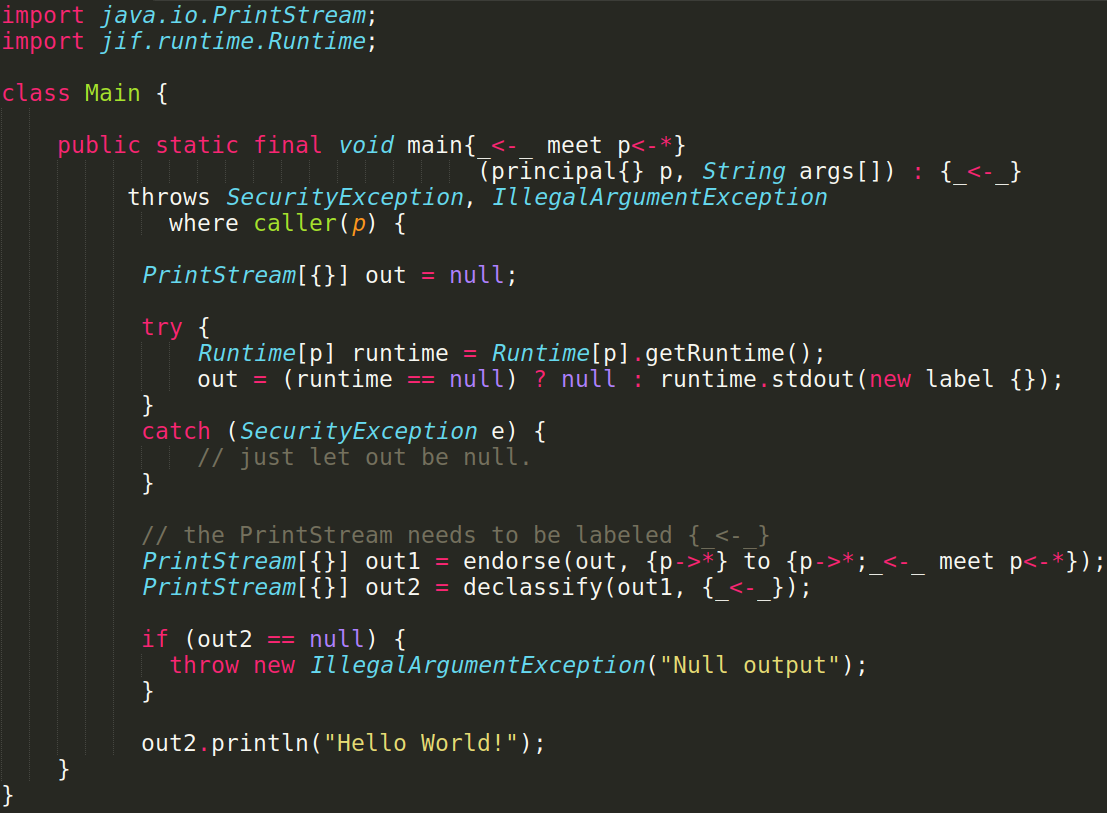
\includegraphics[width=\linewidth]{content/images/jif_helloworld.png}
	\end{figure}
\end{frame}

\begin{frame}{JIF: Static Checking Errors}
	\begin{figure}
		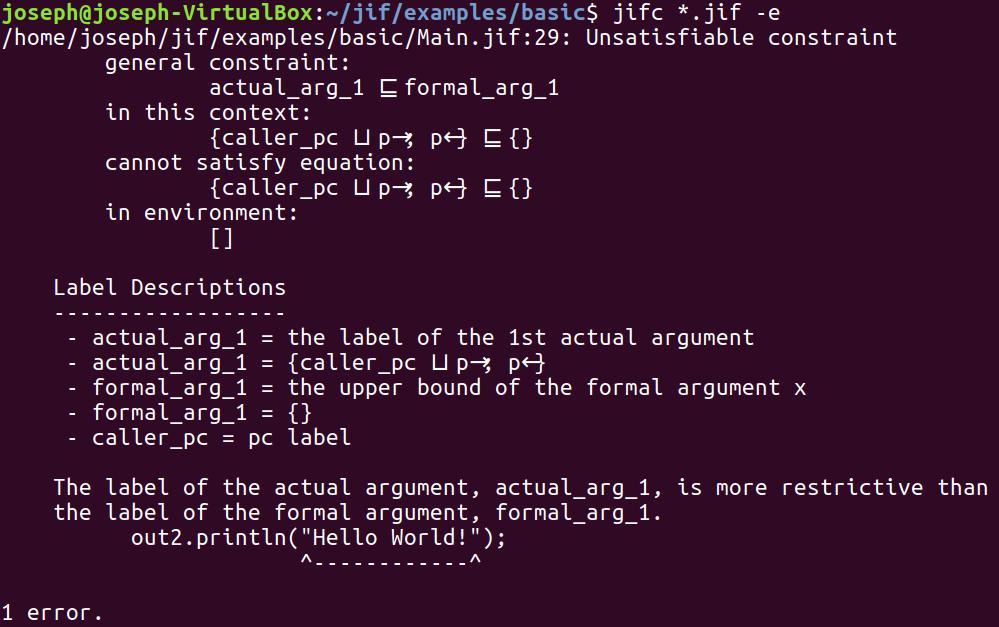
\includegraphics[scale=0.5]{content/images/jif_helloworld_error.png}
		\caption{A JIF compiler error}
	\end{figure}
\end{frame}

\begin{frame}{JIF: Practicality \& Programmer Burden}
	
	JIF's issues:
	
	\begin{itemize}
		\item Inherently complex policies
		\begin{itemize}
			\item Inclusion of integrity controls complicates them further
		\end{itemize}
		\item Programmer burden compounds as complexity increases
		\item Sparse docs, no debugger, misleading compiler errors
		\item Interoperability issues with Java
	\end{itemize}

	While JIF is useful for comparison against other implementations, the burden it imposes seems to make it impractical for real world use.
	
	\note{
		Thus far in my research, JIF's largest problem has proven to be the complexity of its policies and the programmer burden that induces.
		
		JIF inherently places a large cognitive burden on the programmer: the programmer must provide correct policies for flows within the system at every level, which compounds as programs get larger, and as they have to perform more complex tasks, which makes writing modular programs difficult.
		
		While documentation is sparse, and the compiler's error messages often do not correspond to the true information flow problem, these merely exacerbate the core burden issue.
		
		In addition, though Jif has the advantage of being based on Java, interoperability is limited -- features like reflection do not exist, and external libraries require JIF signatures for their interfaces.
		}
	
	
\end{frame}

\begin{frame}[fragile]{LIFTy -- An Alternate Approach}
	
	Liquid Information Flow Types (LIFTy) provides some solutions to these issues, though it is not based on Java. LIFTy provides:
	
	\begin{itemize}
		\item `Policy agnostic' code -- policies specified \textit{once}, separately
		\item Simple, predicate based policies
		\item Automatically adds checks with no programmer effort
		\begin{itemize}
			\item Downside: won't error on a malformed policy
		\end{itemize}
	\end{itemize}
	
	\begin{figure}
		\begin{lstlisting}[escapeinside={(*}{*)}]
getPaperAuthors :: 
		w:World(*$ \rightarrow $*)PaperId(*$ \rightarrow $*)Tagged[User]<(*$ \mathcal{V} $*)=chair w>
showPaper w pid =
	let u = getCurrentUser w
		out = do title (*$ \leftarrow $*) getPaperTitle w pid
						 authors (*$ \leftarrow $*) getPaperAuthors w pid
						 return (title + + ": " + + show authors)
	in print w u out

		\end{lstlisting}
		\caption{`Blind review' LIFTy example \cite{work:lifty}}
	\end{figure}
	
	\note{
		LIFTy is a different information flow-secure language, that provides some solutions to these problems. Specifically, code is \textbf{policy agnostic}, and the policies are simple predicates rather than complex DLM labels.
		
		LIFTy is not Java-based; it is a statically typed $ \lambda $-calculus based language that uses `type driven program repair' to automatically add access checks on confidential data during compilation.
	}
	
\end{frame}

\begin{frame}{Further Exploration}
	The paper introducing LIFTy is still in submission, but it warrants further exploration.
	
	Another implementation that is worthy of study is Paragon -- like JIF, Paragon is Java based, but it uses a more refined policy specification based on predicate-based `flow locks'.
	
	Initial impressions of the language are that while its policy mechanism is more complex than LIFTy's, its reliance on logic-based policies over the DLM may allow it to be far more usable in developing real world applications.
\end{frame}

\begin{frame}{Overall Thoughts So Far}
From my research thus far, the stand out point has been that programmer burden matters. A system which is rigid and complex in its policy specification, and which forces programmers to understand and correctly apply a complex model to the design of their code is inherently less practical than one which allows policies to be specified in a way which is natural.

Ideally, the programmer should be able to derive their policy straight from their program's specification and represent it simply and concisely, freeing them to then build their implementation without having to contort their design around the vagaries of the model the language forces on them.

In addition, the \textit{usefulness} of a model in representing practical security properties seems directly related to the model's flexibility: the DLM, while it allows quite precise and mathematically meaningful policies to be specified, is very difficult to apply to a real world problem like the Calendar example. A logic or predicate-based system, by contrast, can very easily be fit to such a problem.

Usefulness dependent on policy model

Potential for `lighter' solutions (e.g. LIFTy, static analysis tools)
\end{frame}

\begin{frame}{The Plan}

My next step will be to familiarise myself more deeply with LIFTy and Paragon to gain a greater understand of how they compare \textit{in practice} with JIF.

Beyond that, I plan to research further models and potential avenues that future implementations could take. I also plan to use familiarity with several models to come up with a set of criteria with which to perform a more rigorous comparison between and evaluation of each implementation.

\end{frame}
